 \section{Propuesta}
	
\begin{frame}{Propuesta de solución}
% 	\begin{block}{Herramienta para el desarrollador}
% 	\begin{itemize}
% 	  \item Hacer análisis estático del flujo de información de su aplicación.
% 	  \item Anotaciones en el código fuente.
% 	\end{itemize}
% 	\end{block}
	\begin{figure}[t!]
		\begin{center} 
		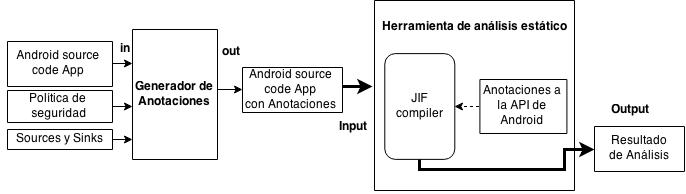
\includegraphics[width=9cm]{desing3Real-2-2.jpg} 
		\end{center}
		\label{fig:desingReal}
	\end{figure}
\end{frame}

\begin{frame}{Política de Seguridad}
	\begin{figure}[t!]
		\begin{center} 
		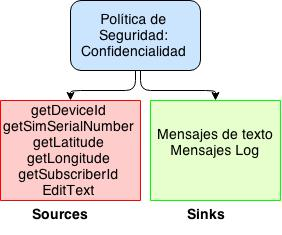
\includegraphics[width=5cm]{Politica.jpg} 
		\end{center}
		\label{fig:desingReal}
	\end{figure}
\end{frame}

\begin{frame}{Anotaciones a la API}
	\begin{figure}[t!]
		\begin{center} 
		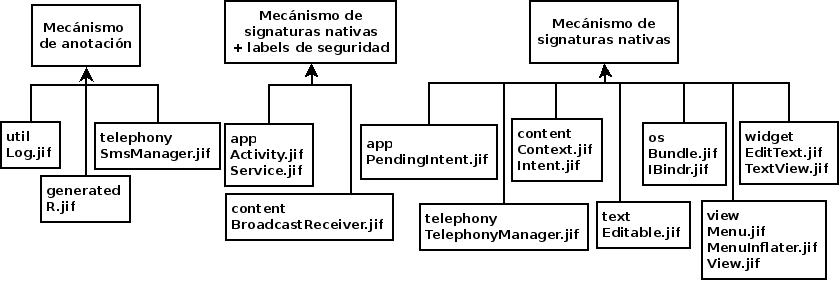
\includegraphics[width=9cm]{annotationsMechanims.jpeg} 
		\end{center}
		\label{fig:desingReal}
	\end{figure}
\end{frame}

\begin{frame}{Lineamientos de Anotación}
	
\end{frame}
